\documentclass[runningheads]{llncs}

\usepackage[T1]{fontenc}
\usepackage{lmodern}
\usepackage{microtype}
\usepackage{amsmath,amssymb,mathtools}
\usepackage{booktabs}
\usepackage{multirow}
\usepackage{array}
\usepackage{graphicx}
\usepackage{algorithm}
\usepackage{algpseudocode}
\usepackage{tikz}
\usetikzlibrary{arrows.meta,positioning,fit,calc,shapes.geometric}
\usepackage[hidelinks]{hyperref}
\usepackage{url}
\usepackage{xspace}
\emergencystretch=2em

\newcommand{\method}{\textsc{EquiSchema}\xspace}
\newcommand{\Dview}{\Delta_{\mathrm{view}}}
\newcommand{\Dseed}{\Delta_{\mathrm{seed}}}
\newcommand{\ESD}{\operatorname{ESD}}
\newcommand{\Cov}{\operatorname{Cov}}
\newcommand{\enc}{\operatorname{Enc}}
\newcommand{\facts}{\mathcal{F}}
\newcommand{\task}{\tau}
\newcommand{\Rone}{\mathrm{R1}}
\newcommand{\Rtwo}{\mathrm{R2}}
\newcommand{\Rthree}{\mathrm{R3}}

\title{Same Facts, Different Predictions?\\\method: Certified Auditing of Storage Invariance and Role Identifiability in Relational Learning}
\titlerunning{\method: Auditing Storage Invariance and Role Identifiability}
\author{Anonymous Author(s)}
\authorrunning{Anonymous Author(s)}
\institute{}

\begin{document}
\maketitle

\begin{abstract}
Relational models are typically evaluated on a single physical schema. Yet a storage refactoring can preserve the same logical facts while changing their distance in the graph. We introduce \method, an audit that combines executable instance-level rewrite certificates and task-integrity contracts with paired predictions, seed-normalized drift, and logical-context diagnostics. The audit treats storage invariance and sensitivity to distinct foreign-key roles as separate properties. In two generated domains, three certified rewrites reduce to three unique context states; LightGBM and a typed message-passing control recover the intended context-loss mechanisms. Raw role interventions and serialization controls distinguish semantic role keys, positional slots, and complete role collapse. A version-pinned source audit identifies a Relational Transformer (RT) role-collision risk without claiming an end-to-end RT failure. We also run a five-seed, budgeted GraphSAGE audit on RelBench's official \texttt{rel-f1/qualifying-position} task. Vertical decomposition lowers sampled fact Jaccard to .701, but normalized excess schema drift is .0157 with a 95\% seed/race-cluster resampling interval of [$-.0721,.1236$]. The interval includes zero, and the ten-epoch models underperform a training-median reference. The real-data experiment demonstrates the audit protocol, but does not establish excess predictive drift or production-model robustness.
\end{abstract}
\keywords{Relational deep learning \and Relational foundation models \and Schema invariance \and Foreign-key roles \and Database normalization \and Robustness auditing}

\section{Introduction}
A relational database can have several physical representations of the same application-level facts. Vertical decomposition, denormalization, and foreign-key (FK) reification can change join paths or graph distances while preserving those facts. A relational deep learning (RDL) pipeline that samples a bounded number of physical hops may therefore retrieve different information for the same target entity. Evaluation on a single schema does not measure that sensitivity.

Semantic roles impose a different requirement. Buyer and seller may reference the same customer table, but exchanging them changes a transaction's meaning. A representation that collapses these predicates can produce the same prediction even when the task requires a different one. We call these two properties \emph{storage invariance} and \emph{role identifiability}.

RelBench standardizes relational prediction tasks~\cite{robinson2024relbench}, while Castor established schema independence as a learning objective~\cite{picado2017schema}. RDB2G-Bench studies graph-modeling choices~\cite{choi2025rdb2g}, and equivalent-schema robustness also arises in Text-to-SQL~\cite{kanchinadam2026schemas}. \method complements these lines with executable instance-level equivalence checks, fixed task contracts, entity-paired predictions, seed baselines, and context diagnostics. The contribution is an audit, not a general theory of schema independence.

\paragraph{Contributions.}
We contribute (i) executable storage-rewrite certificates paired with task-integrity contracts; (ii) entity-paired drift, seed baselines, and logical-context diagnostics; (iii) role-sensitivity controls and a version-pinned representation audit; and (iv) reproducible controlled calibration plus a real-data GraphSAGE audit. The real-data audit can return an inconclusive result when schema drift cannot be separated from fitting noise. Our claims concern the executed instances and protocols, not universal schema independence.

\section{Related Work and Novelty Boundary}\label{sec:related}
\subsection{Database equivalence and metamorphic testing}
Hull formalized relative information capacity between relational schemata \cite{hull1986capacity}. Our executable round-trip certificate is narrower: it checks equivalence for a specific task and instance. Methodologically, \method is also related to metamorphic testing: when a conventional output oracle is unavailable, one tests necessary relations between outputs under transformations \cite{xie2011metamorphic}. Here the metamorphic relation is prediction stability only for certified storage rewrites; semantic role interventions deliberately require sensitivity instead.

\subsection{Schema-independent relational learning}
Picado et al. formalized schema independence for relational learning and showed that conventional learners may change behavior when the same information is represented through decomposition or composition \cite{picado2017schema}. Modern RDL adds bounded sampling, heterogeneous edge types, temporal censoring, and stochastic fitting, motivating prediction-level audits with context diagnostics.

\subsection{Relational database benchmarks and graph construction}
RelBench provides standardized predictive tasks with temporal splits and a reference heterogeneous graph neural network (GNN) pipeline \cite{robinson2024relbench}. RDB2G-Bench systematically varies relational-to-graph modeling and shows that representation choice can materially affect performance \cite{choi2025rdb2g}. These studies show that modeling choices matter. They do not require an inverse certificate for representations of the same logical database instance, and paired prediction consistency for the same entities is not their focus.

\paragraph{Relational models.}
Relational foundation models (RFMs) extend this setting toward transfer. RelGNN introduces composite message passing for challenging relational structures \cite{chen2025relgnn}, and RelGT uses transformer-style processing over relational graph structure \cite{dwivedi2026relgt}. The Relational Transformer (RT) moves toward zero-shot transfer across relational schemas \cite{ranjan2026rt}; RT-J scales pretraining and context-efficient prediction on real relational data \cite{ranjan2026rtj}. RelArena-alpha provides a unified contemporary evaluation environment and strong flattening/model baselines including TabPFN-Rel \cite{hayler2026relarena}.

Mechanistic work on synthetic relational pretraining has begun to use FK interventions to test whether learned predictors actually depend on relational structure \cite{dubey2026synthetic}. That work asks whether pretraining induces relational computation. Given a predictive pipeline, \method tests whether its predictions remain stable under certified storage rewrites and respond to semantic role changes.

\paragraph{Adjacent robustness and task integrity.}
Kanchinadam et al. study large language model (LLM) Text-to-SQL robustness under equivalent schemas \cite{kanchinadam2026schemas}. Query-generation consistency differs from paired predictive consistency and temporal context selection.

Relational Task Generation Language (RTGL) reports temporal inconsistencies in manually authored relational task SQL, including future-activity eligibility in RelBench's \texttt{driver-dnf} \cite{kolesnichenko2026rtgl}. Because task leakage is orthogonal to storage invariance, we make task integrity an explicit precondition for external schema auditing.

\begin{table}[t]
\centering
\caption{Positioning against the closest lines of work. A checkmark means the property is a central evaluated object, not merely possible in the implementation.}
\label{tab:boundary}
\small
\setlength{\tabcolsep}{4.4pt}
\resizebox{\textwidth}{!}{%
\begin{tabular}{lccccc}
\toprule
Work & Eq. cert. & Predictive RDL & Paired pred. & Role ID & Layer diag.\\
\midrule
Castor \cite{picado2017schema} & \checkmark & -- & -- & -- & --\\
RDB2G-Bench \cite{choi2025rdb2g} & -- & \checkmark & -- & -- & --\\
Same Data, Different Schemas \cite{kanchinadam2026schemas} & \checkmark\textsuperscript{$\dagger$} & -- & -- & -- & --\\
FK-intervention study \cite{dubey2026synthetic} & -- & \checkmark & -- & -- & \checkmark\\
\textbf{\method} & \checkmark & \checkmark & \checkmark & \checkmark & \checkmark\\
\bottomrule
\multicolumn{6}{l}{\footnotesize \textsuperscript{$\dagger$} Equivalent-schema construction for Text-to-SQL rather than a database round-trip certificate.}
\end{tabular}%
}
\end{table}

\section{Problem Formulation}\label{sec:formal}
Let $D\in\mathcal{D}(S)$ be a legal database instance under physical schema $S$. A predictive task $\task$ specifies target entities, labels (when observed), one or more temporal cutoffs, and an evaluation metric. Let $A(D,\task;\xi)$ be a complete prediction procedure including preprocessing, neighborhood/context selection, fitting or in-context prediction, and randomness $\xi$. For target entity $e$, let $p_A(e\mid D,\task;\xi)$ denote a score or predictive distribution.

\subsection{Logical facts and certified storage equivalence}
We use $\facts(D)$ to denote a task-relevant logical fact interpretation rather than literal table bytes. A physical rewrite may introduce or remove tables while preserving $\facts(D)$. To make this claim auditable, we require an executable certificate.

\begin{definition}[Rewrite certificate]
A rewrite certificate is $C=(T,U,\phi,\Omega)$ where $T$ maps instances of schema $S$ to schema $S'$, $U$ is an executable inverse, $\phi$ maps target-entity identifiers from $D$ to $T(D)$, and $\Omega$ is a set of admissibility preconditions (keys, functional dependencies, null semantics, row coverage, and temporal conditions). A rewrite is \emph{certified for task $\task$} when, for all checked legal instances satisfying $\Omega$,
\begin{equation}
U(T(D)) \equiv_{\task} D,
\label{eq:roundtrip}
\end{equation}
where $\equiv_{\task}$ requires equality of task-visible logical facts, preservation of the target mapping $\phi$, unchanged labels, and unchanged task cutoffs.
\end{definition}

Certificates encode the inverse's admissibility assumptions. For N:1 denormalization these include the dimension functional dependency and retention of unused members. Verification compares typed keyed rows, or multisets where duplicates matter, and preserves null absence. Temporal joins must use information available at the task cutoff; a future-state snapshot is inadmissible. These conditions enter $\Omega$ and Algorithm~\ref{alg:cert}.

\begin{definition}[Task-integrity contract]\label{def:taskcontract}
For temporal task $\task$, $B=(Q,I,H,\Gamma)$ records the target query, entity-eligibility rule, declared time horizon, and hidden-column policy. It is \emph{time-safe} when eligibility at anchor $t$ uses no information after $t$, labels use only the declared target window, and evaluated keys/labels/cutoffs remain unchanged across certified views. Autocomplete tasks use the analogous row-mask contract. Both $C$ and $B$ must pass before view drift is admissible.
\end{definition}
Task leakage/misalignment is therefore an L0 validity failure, not evidence for or against invariance.

\subsection{Storage invariance}
For a certificate $C$, define a prediction discrepancy $d(\cdot,\cdot)$, such as absolute probability change or hard-label disagreement. To compare schema drift and training noise under the same stochastic coupling, our primary view-drift estimand uses \emph{independent} seeds:
\begin{equation}
\Dview^{\mathrm{ind}}(T)=\mathbb{E}_{\xi\neq\xi'}\frac{1}{|E|}\sum_{e\in E}
 d\!\left(p_A(e\mid D;\xi),p_A(\phi(e)\mid T(D);\xi')\right).
\end{equation}
The same-schema baseline is
\begin{equation}
\Dseed=\mathbb{E}_{\xi\neq\xi'}\frac{1}{|E|}\sum_{e\in E}
 d\!\left(p_A(e\mid D;\xi),p_A(e\mid D;\xi')\right),
\end{equation}
and define excess schema drift (ESD) as
\begin{equation}
\ESD^{\mathrm{ind}}(T)=\Dview^{\mathrm{ind}}(T)-\Dseed.
\label{eq:esd}
\end{equation}
Thus both terms average over the same ordered independent-seed pairs. We additionally retain matched-seed $\Dview^{\mathrm{pair}}$ as a sensitivity diagnostic because it removes one source of fitting noise, but it is not subtracted from an independently seeded baseline. Positive ESD means view changes add disagreement beyond refitting noise; ESD near zero means the audit does not detect excess drift. For the controlled hard-label results, 2,000 bootstrap replicates resample fitted seeds and test entities. The same seed weights are reused across views and both ESD terms; pairs with equal original seed IDs remain excluded. Thus the 20 ordered pairs are not treated as 20 independent fits. These intervals condition on the generated database and have limited resolution with five seeds.

For classification we also report area under the receiver operating characteristic curve (AUROC), calibration, and \emph{worst-view performance}:
\begin{equation}
M_{\mathrm{worst}}=\begin{cases}
\min_{V\in\mathcal{V}}M(A,V), & \text{higher is better},\\
\max_{V\in\mathcal{V}}M(A,V), & \text{lower is better}.
\end{cases}
\end{equation}
where $\mathcal{V}$ contains the original and certified views.

\subsection{Role identifiability}
Let $r_1$ and $r_2$ be two semantically distinct FK roles into the same parent table. A role intervention $\rho$ swaps or otherwise changes these predicates while preserving the referenced entity values. Unlike a storage rewrite, $\rho$ is \emph{not} label preserving in general; it changes logical semantics.

\begin{definition}[Role identifiability]
For a task where role changes can affect the target, a predictor is role identifiable on a pair $(x,\rho(x))$ if its response is directionally consistent with the verified role-conditioned target contrast. We report directional concordance and, when counterfactual target flips are available, the correct-flip rate.
\end{definition}

\begin{lemma}[Role-collision limitation]\label{lem:collision}
If an encoder maps a role-sensitive pair to the same representation, $\enc(x)=\enc(\rho(x))$, then any deterministic predictor $g\circ\enc$ returns the same prediction for the pair. Consequently it cannot be correct on both members whenever their Bayes-optimal decisions differ.
\end{lemma}
\begin{proof}
Equality of encodings implies $g(\enc(x))=g(\enc(\rho(x)))$. If the optimal labels differ, at least one equal decision is wrong. The statement is architectural and does not depend on the choice of $g$.
\end{proof}
The lemma provides a diagnostic: a representation collision can be tested as an explanation before interpreting end-to-end performance.

\section{The \method Audit}\label{sec:method}
\subsection{Certified rewrite family}
We separate core storage rewrites from metadata perturbations.

\paragraph{R1: lossless vertical decomposition (1:1).}
For a keyed relation $R(K,A,B)$, create $R_A(K,A)$ and $R_B(K,B)$ with $K$ unique in both. The inverse is a one-to-one join on $K$. This rewrite is useful because it can increase the physical distance between an entity and an attribute without changing the logical fact.

\paragraph{R2: N:1 denormalization.}
For fact relation $F(\ldots,K_D,\ldots)$ referencing dimension $D(K_D,Z)$, copy $Z$ into $F$. The certificate requires $K_D\rightarrow Z$, explicit treatment of null FKs, and preservation of dimension rows needed for exact inversion. We recommend retaining a key-only dimension remainder or an auxiliary manifest for unused dimension members rather than pretending that an ordinary left join is always invertible.

\paragraph{R3: FK reification.}
Replace an FK column with a role-labelled link relation $L(K_F,r,K_P)$ and remove the direct edge. The inverse pivots or selects the unique $(K_F,r)$ link back into the original FK column. Null FKs are represented by missing role links plus a null manifest where needed for exact round trip.

\paragraph{Metadata perturbations.}
Renaming a table or column while preserving relational algebra is \emph{not} included in the core storage-invariance family when a model intentionally consumes schema text. Such tests measure metadata robustness, a separate property. This distinction avoids declaring meaningful schema semantics ``irrelevant'' by fiat.

\begin{algorithm}[t]
\caption{Certificate verification and paired-entity manifest construction}
\label{alg:cert}
\begin{algorithmic}[1]
\Require Database $D$, task $\task$, rewrite $T$, inverse $U$, entity map $\phi$, preconditions $\Omega$
\Ensure Verified transformed database $D^{\prime}$ and pairing manifest $P$, or \textsc{Reject}
\State Validate keys, FKs, functional dependencies, null policy, and temporal assumptions in $\Omega$
\If{any precondition fails} \State \Return \textsc{Reject} \EndIf
\State $D^{\prime}\gets T(D)$
\State $\widehat D\gets U(D^{\prime})$
\State Canonicalize every task-visible relation (types, key order, nulls, duplicate semantics)
\If{$\operatorname{hash}_{\task}(\widehat D)\neq\operatorname{hash}_{\task}(D)$}
    \State \Return \textsc{Reject}
\EndIf
\State Verify task contract $B$: cutoff(s), eligibility/history bounds, target window, hidden columns
\State Hash evaluated entity--time keys and labels; require equality across $D$ and $D^{\prime}$
\State Verify $\phi$ is one-to-one over evaluated target entities
\If{any task-integrity invariant fails} \State \Return \textsc{Reject} \EndIf
\State Emit pairing manifest $P=\{(e,\phi(e)):e\in E_{\task}\}$ together with logical-fact identifiers for context comparison
\State \Return $(D^{\prime},P,\textsc{Verified})$
\end{algorithmic}
\end{algorithm}

\subsection{Logical context and layerwise diagnosis}
Let $N_A(e,D)$ be the set of logical fact identifiers actually made visible to the predictor for entity $e$ after preprocessing/sampling. For a matched pair we compute logical-context coverage
\begin{equation}
\Cov(e;D,D')=
\frac{|N_A(e,D)\cap \psi^{-1}(N_A(\phi(e),D'))|}
{|N_A(e,D)\cup \psi^{-1}(N_A(\phi(e),D'))|},
\label{eq:coverage}
\end{equation}
where $\psi$ maps transformed records back to logical fact IDs; coverage is one when both sets are empty. This enables four diagnostic layers:
\begin{description}
    \item[L0 -- certificate failure:] the rewrite is not task-equivalent; no invariance claim is valid.
    \item[L1 -- encoding collision:] two semantically distinct role configurations become the same representation (Lemma~\ref{lem:collision}).
    \item[L2 -- context-selection mismatch:] the views are equivalent, but bounded physical-hop/fanout retrieval exposes different logical facts; $\Cov<1$.
    \item[L3 -- predictor/training instability:] logical context is coupled ($\Cov\approx1$), yet predictions still differ beyond seed noise.
\end{description}
The layers help distinguish an encoder collision from a sampling mismatch caused by a change in physical paths.

\subsection{Mitigations}
We evaluate explicit role-keyed channels and restoration of complete logical context. In the controlled domains, the latter is a hand-specified canonical flattened view. Training-time schema augmentation and a certificate-aware logical sampler remain \emph{unevaluated extensions}. A logical sampler would need to improve the quality--latency/memory frontier over canonical materialization to justify its use.

\section{System and Source-Code Audit}\label{sec:audit}
\subsection{A concrete role-representation asymmetry}
We audited version-pinned public code paths used to construct relational neighborhoods. In the RelBench heterogeneous graph builder, an FK edge type is constructed as
the relation type \texttt{f2p\_FK} (where \texttt{FK} is the originating FK column), with a correspondingly named reverse edge \cite{relbenchcode2026}. Thus two columns in the same child table that reference the same parent table remain distinct relation types.

In the examined RT/RT-J-compatible Rust preprocessing path, the input manifest maps FK column names to parent tables, but each serialized structural edge contains the neighboring node index, parent table identity/type, and timestamp; the edge structure does not store the originating FK-column identifier \cite{rtcode2026}. During construction, distinct FK columns that target the same parent table therefore contribute edges carrying the same parent-table type. This is an explicit L1 collision risk when downstream attention cannot reconstruct the original role from other evidence.

This source-code observation is not an end-to-end performance result: other features or table context may correlate with role. The representation hypothesis can be tested by adding or removing a role token while holding the rest of the system fixed.

\subsection{Natural repeated-role schema: \texttt{rel-salt}}
RelBench v2/v3 includes the enterprise \texttt{rel-salt} dataset. Its sales-item relation contains four customer FK roles (sold-to, ship-to, bill-to, and payer), all referencing \texttt{customer} \cite{relbenchdata2026}. The repeated roles arise naturally, making the dataset suitable for a role-identifiability audit.

Repeated roles alone do not establish a label effect. A task-level experiment must also show that role-conditioned information predicts the selected target under the official cutoff.

\begin{figure}[t]
\centering
\resizebox{0.98\textwidth}{!}{%
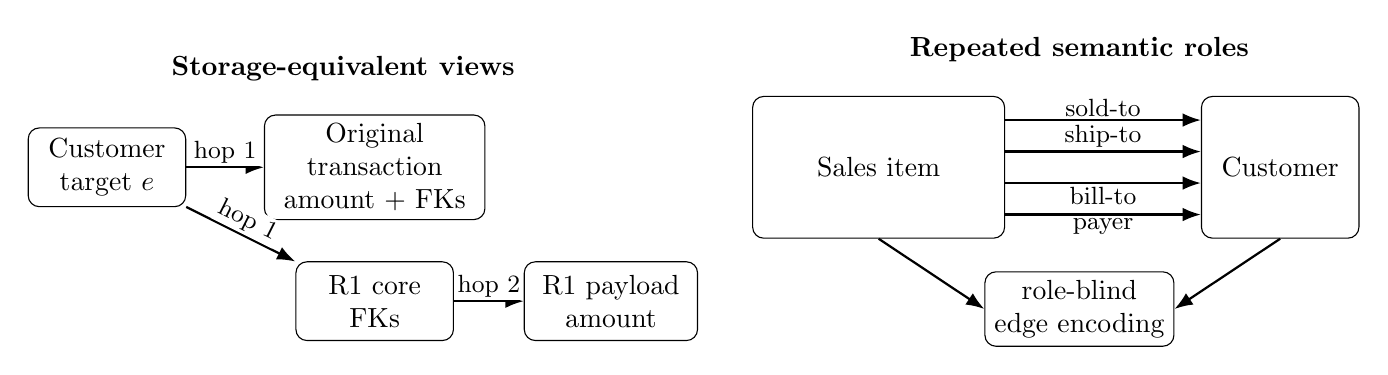
\begin{tikzpicture}[font=\normalsize,>=Latex,
box/.style={draw,rounded corners,align=center,minimum height=10mm,inner sep=3pt},
arr/.style={->,thick},
lab/.style={fill=white,inner sep=1pt,font=\small}]
% left panel: physical distance changes
\node[box,minimum width=20mm] (cust) at (0,0) {Customer\\target $e$};
\node[box,minimum width=28mm] (tx) at (3.4,0) {Original\\transaction\\amount + FKs};
\draw[arr] (cust) -- node[lab,above]{hop 1} (tx);
\node[box,minimum width=20mm] (core) at (3.4,-1.7) {R1 core\\FKs};
\node[box,minimum width=22mm] (payload) at (6.4,-1.7) {R1 payload\\amount};
\draw[arr] (cust) -- node[lab,above,sloped]{hop 1} (core);
\draw[arr] (core) -- node[lab,above]{hop 2} (payload);
\node[font=\bfseries] at (3.0,1.25) {Storage-equivalent views};
% right panel: repeated roles
\node[box,minimum width=32mm,minimum height=18mm] (item) at (9.8,0) {Sales item};
\node[box,minimum width=20mm,minimum height=18mm] (customer) at (14.9,0) {Customer};
\draw[arr] ([yshift=6mm]item.east) -- node[lab,above]{sold-to} ([yshift=6mm]customer.west);
\draw[arr] ([yshift=2mm]item.east) -- node[lab,above]{ship-to} ([yshift=2mm]customer.west);
\draw[arr] ([yshift=-2mm]item.east) -- node[lab,below]{bill-to} ([yshift=-2mm]customer.west);
\draw[arr] ([yshift=-6mm]item.east) -- node[lab,below]{payer} ([yshift=-6mm]customer.west);
\node[font=\bfseries] at (12.35,1.5) {Repeated semantic roles};
\node[box,minimum width=24mm,minimum height=7mm] (blind) at (12.35,-1.8) {role-blind\\edge encoding};
\draw[arr] (item.south) -- (blind.west);
\draw[arr] (customer.south) -- (blind.east);
\end{tikzpicture}%
}
\caption{Two complementary failure mechanisms. Left: a certified rewrite can preserve facts while changing physical distance, producing an L2 context-selection mismatch. Right: repeated FKs into the same parent table carry different semantics; collapsing their role identity creates an L1 representation collision.}
\label{fig:overview}
\end{figure}

\section{Controlled Experimental Calibration}\label{sec:controlled}
The generated study \emph{calibrates} the audit using known logical facts and certificates. Its sampler is intentionally simple, so the study does not show whether a production GNN or RFM fails on these rewrites.

\subsection{Domains, certificates, and representation states}
We generate two independent domains, each with 3,000 customers, 240 merchants, and 45,000 transactions. A transaction contains buyer, seller, and merchant FKs, amount, and time. The balanced target depends on an entity attribute plus buyer/seller-conditioned amount, count, and merchant-risk aggregates with opposing signs. Synth-B is heavier tailed than Synth-A.

We execute R1 (vertical decomposition), R2 (N:1 denormalization with an unused-dimension remainder), and R3 (role-labelled FK reification), run $U(T(D))$, canonicalize rows, and verify exact equality; SHA-256 round-trip hashes are emitted. Under the bounded physical-path sampler, however, several schema views intentionally induce the \emph{same feature state}. We therefore do not count those rows as independent replications. State completeness below counts three transaction-contribution channels. Paired Jaccard additionally includes the entity attribute; merchant-risk IDs denote joined transaction contributions, not distinct merchant cells. The controlled states are
\begin{itemize}
    \item $S_{\mathrm{low}}$: structure only (coverage .33; R1$_1$, R3$_1$),
    \item $S_{\mathrm{mid}}$: structure + amount (coverage .67; $O_1$, R3$_2$),
    \item $S_{\mathrm{full}}$: structure + amount + merchant risk (coverage 1; $O_2$, R1$_2$, R2$_1$/R2$_2$, R3$_3$).
\end{itemize}
R1 therefore realizes $S_{\mathrm{mid}}\!\to S_{\mathrm{low}}$, R2 realizes $S_{\mathrm{mid}}\!\to S_{\mathrm{full}}$, and the chosen R3 stress realizes the reverse $S_{\mathrm{full}}\!\to S_{\mathrm{mid}}$. The latter two share the same unordered representation pair, so equality of their raw hard-disagreement rates is expected rather than evidence from two independent mechanisms.

\subsection{Models and protocol}
\paragraph{Canonical-flat LightGBM.} LightGBM~\cite{ke2017lightgbm} receives the materialized relational aggregates plus the entity feature. At $S_{\mathrm{full}}$ this is an explicit canonical flattening baseline (hand specified, not an automated Deep Feature Synthesis implementation). We use 130 trees, learning rate .04, at most 15 leaves, depth at most 5, subsampling, and seeds $\{11,23,37,51,71\}$.

\paragraph{Typed message-passing neural network (TypedMPNN).} The neural control applies separate buyer/seller linear message maps before a two-layer head. Each role message contains amount, structural count, and merchant-risk aggregates. We use AdamW, binary cross entropy, early stopping on validation AUROC, and the same seeds. No view-specific payload mask is applied; feature availability follows the physical-path traversal.

All views share entity splits. Preprocessing is fitted only on training entities in the complete original state and then frozen across views. The latent oracle retains its separate, fixed population transformation defining the data generator. Table~\ref{tab:auc} reports each \emph{unique} controlled state once.

\begin{table}[t]
\centering
\caption{Unique controlled representation states (AUROC, mean $\pm$ std over five seeds). Duplicate schema views mapping to the same state are listed rather than re-counted as independent evidence.}
\label{tab:auc}
\scriptsize
\setlength{\tabcolsep}{2.2pt}
\begin{tabular}{llccccc}
\toprule
State & Views & Cov. & \multicolumn{2}{c}{Synth-A} & \multicolumn{2}{c}{Synth-B}\\
 & & & LGBM & MPNN & LGBM & MPNN\\
\midrule
% BEGIN GENERATED controlled_performance
$S_{\rm low}$ & R1$_1$, R3$_1$ & .33 & 0.845$\pm$0.000 & 0.848$\pm$0.006 & 0.839$\pm$0.001 & 0.794$\pm$0.032\\
$S_{\rm mid}$ & $O_1$, R3$_2$ & .67 & 0.914$\pm$0.001 & 0.921$\pm$0.003 & 0.883$\pm$0.001 & 0.884$\pm$0.004\\
$S_{\rm full}$ & $O_2$, R1$_2$, R2$_1$/R2$_2$, R3$_3$ & 1.00 & 0.955$\pm$0.001 & 0.970$\pm$0.002 & 0.899$\pm$0.001 & 0.910$\pm$0.006\\
% END GENERATED controlled_performance
\bottomrule
\end{tabular}
\end{table}

\subsection{Seed-matched and independent-seed drift}
Table~\ref{tab:drift} makes the primary comparison statistically symmetric: both $\Dview^{\rm ind}$ and $\Dseed$ average the same 20 ordered independent-seed pairs. ESD intervals use the paired seed/entity bootstrap described above. The intervals exclude zero for every reported transition. R2 and R3 remain directionally different audits but share the same unordered $S_{\rm mid}/S_{\rm full}$ representation pair; they must not be interpreted as two independent replications.

\begin{table}[t]
\centering
\caption{Hard-label drift in percentage points using independent-seed coupling. ESD is $\Dview^{\rm ind}-\Dseed$; brackets are seed/entity-bootstrap 95\% resampling intervals.}
\label{tab:drift}
\scriptsize
\setlength{\tabcolsep}{2.7pt}
\begin{tabular}{llcrrr}
\toprule
Model & Dom. & Transition & $\Dseed$ & $\Dview^{\rm ind}$ & ESD [95\% CI]\\
\midrule
% BEGIN GENERATED controlled_drift
\multirow{6}{*}{LightGBM} & A & mid$\to$low (R1) & 1.87 & 20.41 & 18.54 [16.03,21.26]\\
 & A & mid$\to$full (R2) & 1.87 & 11.42 & 9.56 [7.63,11.54]\\
 & A & full$\to$mid (R3) & 2.09 & 11.42 & 9.33 [7.39,11.36]\\
 & B & mid$\to$low (R1) & 2.62 & 14.42 & 11.80 [9.66,14.00]\\
 & B & mid$\to$full (R2) & 2.62 & 8.58 & 5.96 [4.33,7.51]\\
 & B & full$\to$mid (R3) & 2.96 & 8.58 & 5.62 [4.04,7.28]\\
\midrule
\multirow{6}{*}{TypedMPNN} & A & mid$\to$low (R1) & 3.02 & 33.82 & 30.80 [19.89,39.97]\\
 & A & mid$\to$full (R2) & 3.02 & 13.57 & 10.54 [8.46,12.62]\\
 & A & full$\to$mid (R3) & 3.09 & 13.57 & 10.48 [8.53,12.51]\\
 & B & mid$\to$low (R1) & 4.02 & 24.38 & 20.36 [11.15,28.04]\\
 & B & mid$\to$full (R2) & 4.02 & 10.83 & 6.81 [5.09,8.76]\\
 & B & full$\to$mid (R3) & 5.31 & 10.83 & 5.52 [3.75,7.42]\\
% END GENERATED controlled_drift
\bottomrule
\end{tabular}
\end{table}

\subsection{Coverage sanity check}
The sampler determines which logical components are reachable, so a monotone coverage curve is partly a consequence of its construction. Figure~\ref{fig:coverage} uses the curve as a calibration check: on R1 with two-hop traversal, first-hop fanout varies the measured coverage while everything else is fixed. We plot matched-seed view disagreement separately for each generated domain, with seed/entity bootstrap intervals for that same paired estimand. The x-axis is paired contribution-fact Jaccard, rather than the fraction of full context. Disagreement falls toward zero as the coupled representations become identical at coverage one. That endpoint is expected by construction and checks the metric and sampler coupling.

\begin{figure}[t]
\centering
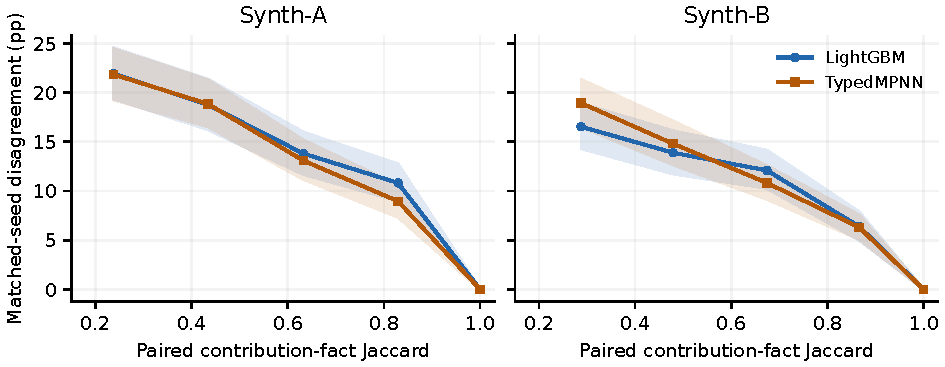
\includegraphics[width=.95\textwidth]{figures/coverage_ablation_v8.pdf}
\caption{Calibration of contribution-fact coverage. First-hop fanout under R1 changes paired Jaccard; bands are within-domain seed/entity-bootstrap 95\% intervals for matched-seed disagreement. The zero endpoint at coverage one is a deterministic sanity check of the coupled representation, not external evidence of invariance.}
\label{fig:coverage}
\end{figure}

\subsection{Role controls beyond the trivial collapsed baseline}
A buyer/seller intervention swaps the raw transaction FKs and recomputes aggregates under frozen preprocessing, preserving referenced entities and non-role attributes. The collapsed control sums raw role contributions before fitting its own train-only preprocessing, preventing role-specific scales from reintroducing role information. The latent generator supplies the expected direction. A fully collapsed encoding is invariant by construction and therefore remains a negative control, not substantive evidence. We add an intermediate \emph{anonymous-slot} control: buyer/seller channels stay separate but the encoder has no semantic role key and relies only on stable slot order. It responds to role swaps as strongly as the role-keyed model when ordering is stable, yet a role-preserving serialization-order permutation causes 68.4--77.4\% hard-label disagreement. In contrast, the role-keyed loader canonicalizes by role label and is invariant to that physical ordering change.

\begin{table}[t]
\centering
\caption{Role controls (\%, five-seed mean). Swap concordance tests a semantic buyer/seller intervention; order drift tests a role-preserving physical slot permutation.}
\label{tab:role}
\scriptsize
\setlength{\tabcolsep}{3.0pt}
\begin{tabular}{llrrrr}
\toprule
Model & Encoding & \multicolumn{2}{c}{Swap concord.} & \multicolumn{2}{c}{Order drift}\\
 & & A & B & A & B\\
\midrule
% BEGIN GENERATED controlled_role
LightGBM & role-keyed & 93.93 & 94.44 & 0.00 & 0.00\\
LightGBM & anonymous-slot & 93.93 & 94.44 & 77.38 & 68.38\\
LightGBM & collapsed & 0.00 & 0.00 & 0.00 & 0.00\\
TypedMPNN & role-keyed & 98.36 & 97.24 & 0.00 & 0.00\\
TypedMPNN & anonymous-slot & 98.36 & 97.24 & 77.20 & 71.00\\
TypedMPNN & collapsed & 0.00 & 0.00 & 0.00 & 0.00\\
% END GENERATED controlled_role
\bottomrule
\end{tabular}
\end{table}

\subsection{What this calibration can and cannot establish}
The audit detects the controlled loss or gain of logical context and distinguishes semantic role keys, anonymous positional slots, and complete role collapse. It does \emph{not} establish that R1--R3 have distinct end-to-end effects in production systems: in this calibration they reduce to three feature states, and two stress directions share the same unordered state pair. Likewise, the role source audit remains a hypothesis until an RT-family behavioral ablation is executed. The canonical full-context state evaluates one simple mitigation; training-time schema augmentation and a certificate-aware sampler remain untested. L0 is exercised by the artifact task-contract linter and the runtime admission checks in Sec.~\ref{sec:external}; this paper does not intentionally manufacture an L3 failure.

\section{Real-Data Audit: \texttt{rel-f1}}\label{sec:external}
We executed the official autocomplete regression task \texttt{qualifying-position}, using pinned RelBench code and data manifests~\cite{relbenchcode2026,relbenchdata2026}. The task uses normalized mean absolute error (NMAE). Its 9,815 target rows comprise 2,228 training, 1,854 validation, and 5,733 test entities. Target keys, timestamps, labels, and the hidden \texttt{qualifying.position} column are fixed across views. R1 decomposes the 26,080-row \texttt{results} relation into FK/time core and attribute payload tables, with copied time metadata and an exact typed round trip. Runtime checks reject sampled nodes after the target cutoff, including future race outcomes that could expose a qualifying-position proxy through \texttt{results.grid}.

\paragraph{Budgeted reference pipeline.}
We use RelBench's heterogeneous GraphSAGE implementation~\cite{hamilton2017graphsage}: two layers, 32 channels, fanouts [32,16], batch size 512, Adam at .005, and ten epochs with validation-NMAE checkpoint selection. Each view is retrained using seeds $\{11,23,37,51,71\}$. This reduced configuration is an audit case study, not a leaderboard reproduction. Graph feature materialization follows the transductive autocomplete reference pipeline on the masked full database; target labels are excluded. Evaluation sampling is fixed across fits. Native NMAE and regression drift both use the training-target standard deviation, 6.6389. Resampling uses shared seed weights and race clusters; five seeds and shared drivers across races limit inferential precision.

\begin{table}[t]
\centering
\caption{Executed RelBench audit. NMAE is lower-is-better; drift is normalized by training-target standard deviation. Intervals are conditional seed/race-cluster resampling intervals.}
\label{tab:real}
\small
\begin{tabular}{lr}
\toprule
Quantity & Value\\
\midrule
% BEGIN GENERATED real_results
Original GraphSAGE NMAE, mean $\pm$ std & 0.9000 $\pm$ 0.0230\\
R1 GraphSAGE NMAE, mean $\pm$ std & 0.8864 $\pm$ 0.0297\\
Training-median reference NMAE & 0.8107\\
Mean paired fact Jaccard & 0.7006\\
Same-schema independent-seed drift & 0.0745\\
Cross-view independent-seed drift & 0.0902\\
ESD [95\% interval] & 0.0157 [$ -0.0721,0.1236$]\\
% END GENERATED real_results
\bottomrule
\end{tabular}
\end{table}

\paragraph{Outcome and canonical control.}
Table~\ref{tab:real} shows context mismatch but no resolved excess predictive drift: the ESD interval includes zero. Both trained configurations underperform the training-median reference, so this result cannot establish invariance of well-fitted production models. Reconstructing the original schema restores its keyed rows, edge topology, and field mapping. Actual CPU inference using the original checkpoints differs from GPU predictions by at most $1.13\!\times\!10^{-6}$ in mean absolute prediction per seed (maximum individual difference $1.74\!\times\!10^{-4}$), consistent with numerical roundoff. This oracle inverse control is not an automated logical sampler or a separate L3 identification experiment. Measured function execution, including dependency installation, took 313 seconds; the experiment process peaked at 3.86 GiB RAM and 1.03 GiB allocated GPU memory.

\section{Discussion and Limitations}
The controlled calibration detects known context changes and separates semantic role keys from positional or collapsed encodings. These results do not establish widespread production failures. On the real task, measurable context loss coexists with an ESD interval spanning zero and weak predictive performance under the fixed training budget. The audit can report this inconclusive outcome; it does not show that physical refactoring is harmless.

External evidence is limited to one database, task, model configuration, and rewrite. Five fitted seeds provide limited uncertainty resolution; shared entities and relational dependencies further constrain resampling interpretations. Controlled intervals condition on two generated databases, and their contribution-level coverage differs from base-table fact coverage on RelBench. The RT source audit establishes a collision risk only; an RT behavioral ablation and a naturally role-sensitive \texttt{rel-salt} task remain future work. R2 requires its unused-dimension remainder, and metadata renaming remains outside core invariance when schema text is consumed. Neither training-time schema augmentation nor a certificate-aware logical sampler is evaluated, and no L3 effect-size claim is made.

\section{Reproducibility and Artifact}
The anonymized supplementary artifact contains executable R1--R3/SHA-256 certificates, five-seed runs, independent-seed/bootstrap analysis, role controls, ablation comma-separated-value (CSV) files, a task-contract linter, figures, and a pinned RelBench runbook. The real-data package includes ten checkpoints, ordered per-target predictions, canonical CPU outputs, version locks, task and rewrite hashes, sampler settings, and cost-envelope receipts. Tables and plots are regenerated from the saved outputs.

\section{Conclusion}
\method combines instance-level rewrite certificates, fixed task contracts, paired predictions, seed baselines, and context diagnostics. Controlled calibration recovers intended context and role mechanisms. A version-pinned RelBench run measures context mismatch but does not resolve predictive drift beyond seed noise under its limited training budget. The result separates a measured change in context from a predictive effect that the experiment cannot resolve.

\section*{Declarations}
\paragraph{Data availability.} Controlled data are generated by the reproduction code. Public RelBench data and task manifests are identified by pinned revisions in the artifact.
\paragraph{Ethics.} This study uses generated and public benchmark data; no new human-participant data were collected.
\paragraph{Author contributions.} Individual CRediT roles are withheld in this anonymous manuscript.
\paragraph{Funding.} This research received no external funding.
\paragraph{Conflict of interest.} The authors declare no conflict of interest.

\bibliographystyle{splncs04}
\bibliography{references}

\end{document}
